\documentclass[tikz, border=8pt]{standalone}
\usepackage{tikz}
\usetikzlibrary{arrows.meta, calc}

\begin{document}
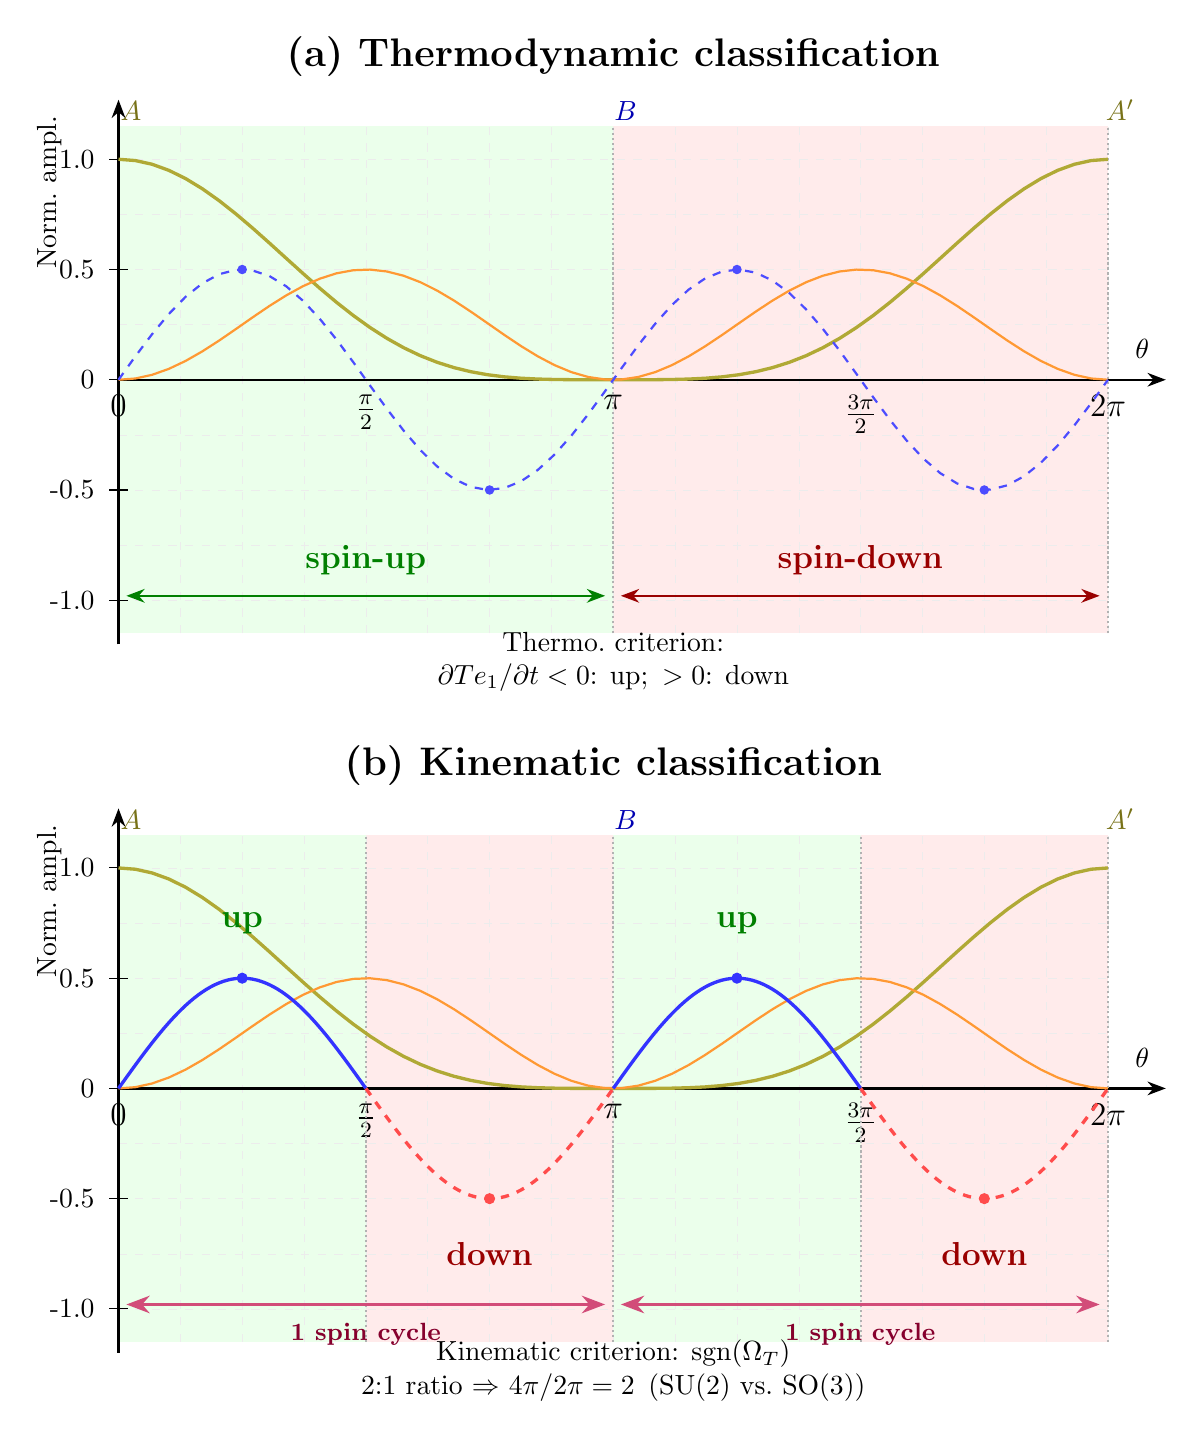
\begin{tikzpicture}[>=Stealth, x=2.0cm, y=2.8cm]

\def\ylo{-1.15}
\def\yhi{1.15}
\def\xmax{6.28318}

%% UPPER PANEL (a): Thermodynamic classification
\node[font=\Large\bfseries, anchor=south] at (3.14159, \yhi+0.18)
    {(a) Thermodynamic classification};
\fill[green!8] (0, \ylo) rectangle (3.14159, \yhi);
\fill[red!8]   (3.14159, \ylo) rectangle (\xmax, \yhi);
\draw[gray!15, xstep=0.3927, ystep=0.25, dashed, very thin]
    (0,\ylo) grid (\xmax, \yhi);
\draw[thick, ->] (0,0) -- (6.65,0);
\draw[thick, ->] (0,\ylo-0.05) -- (0,\yhi+0.12);
\node[font=\normalsize, anchor=south] at (6.5, 0.05) {$\theta$};
\node[font=\normalsize, anchor=south, rotate=90] at (-0.30, 0.85) {Norm.\ ampl.};
\foreach \y in {-1.0, -0.5, 0, 0.5, 1.0} {
    \draw (0.06,\y) -- (-0.06,\y);
    \node[left, font=\normalsize] at (-0.09,\y) {\y};
}
\node[below, font=\large, yshift=-2pt] at (0,       0) {$0$};
\node[below, font=\large, yshift=-2pt] at (1.5708,  0) {$\frac{\pi}{2}$};
\node[below, font=\large, yshift=-2pt] at (3.14159, 0) {$\pi$};
\node[below, font=\large, yshift=-2pt] at (4.7124,  0) {$\frac{3\pi}{2}$};
\node[below, font=\large, yshift=-2pt] at (6.28318, 0) {$2\pi$};
\draw[gray!60, densely dotted, thick] (3.14159,\ylo) -- (3.14159,\yhi);
\draw[gray!60, densely dotted, thick] (6.28318,\ylo) -- (6.28318,\yhi);
\node[font=\normalsize, olive!80!black, above] at (0.08,    \yhi-0.02) {$A$};
\node[font=\normalsize, blue!70!black,  above] at (3.22,    \yhi-0.02) {$B$};
\node[font=\normalsize, olive!80!black, above] at (6.36,    \yhi-0.02) {$A'$};
\draw[olive!70, very thick, domain=0:\xmax, samples=60]
    plot (\x, {(cos(\x * 180 / 3.14159 / 2))^4});
\draw[orange!80, thick, domain=0:\xmax, samples=60]
    plot (\x, {0.5*(sin(\x * 180 / 3.14159))^2});
\draw[blue!70, thick, dashed, domain=0:\xmax, samples=60]
    plot (\x, {0.5*sin(2 * \x * 180 / 3.14159)});
\filldraw[blue!70] (0.7854,  0.5) circle (1.5pt);
\filldraw[blue!70] (2.3562, -0.5) circle (1.5pt);
\filldraw[blue!70] (3.9270,  0.5) circle (1.5pt);
\filldraw[blue!70] (5.4978, -0.5) circle (1.5pt);
\node[font=\large\bfseries, green!50!black] at (1.57, -0.82) {spin-up};
\node[font=\large\bfseries, red!60!black]   at (4.71, -0.82) {spin-down};
\draw[<->, green!50!black, thick] (0.05, -0.98) -- (3.09, -0.98);
\draw[<->, red!60!black,   thick] (3.19, -0.98) -- (6.23, -0.98);
\node[font=\normalsize, align=center] at (3.14159, -1.28)
    {Thermo.\ criterion:\\$\partial Te_1/\partial t < 0$: up;\enspace $> 0$: down};

%% LOWER PANEL (b): Kinematic classification
\begin{scope}[yshift=-9.0cm]
\node[font=\Large\bfseries, anchor=south] at (3.14159, \yhi+0.18)
    {(b) Kinematic classification};
\fill[green!8]  (0,       \ylo) rectangle (1.5708,  \yhi);
\fill[red!8]    (1.5708,  \ylo) rectangle (3.14159, \yhi);
\fill[green!8]  (3.14159, \ylo) rectangle (4.7124,  \yhi);
\fill[red!8]    (4.7124,  \ylo) rectangle (\xmax,   \yhi);
\draw[gray!15, xstep=0.3927, ystep=0.25, dashed, very thin]
    (0,\ylo) grid (\xmax, \yhi);
\draw[thick, ->] (0,0) -- (6.65,0);
\draw[thick, ->] (0,\ylo-0.05) -- (0,\yhi+0.12);
\node[font=\normalsize, anchor=south] at (6.5, 0.05) {$\theta$};
\node[font=\normalsize, anchor=south, rotate=90] at (-0.30, 0.85) {Norm.\ ampl.};
\foreach \y in {-1.0, -0.5, 0, 0.5, 1.0} {
    \draw (0.06,\y) -- (-0.06,\y);
    \node[left, font=\normalsize] at (-0.09,\y) {\y};
}
\node[below, font=\large, yshift=-2pt] at (0,       0) {$0$};
\node[below, font=\large, yshift=-2pt] at (1.5708,  0) {$\frac{\pi}{2}$};
\node[below, font=\large, yshift=-2pt] at (3.14159, 0) {$\pi$};
\node[below, font=\large, yshift=-2pt] at (4.7124,  0) {$\frac{3\pi}{2}$};
\node[below, font=\large, yshift=-2pt] at (6.28318, 0) {$2\pi$};
\foreach \xb in {1.5708, 3.14159, 4.7124, 6.28318} {
    \draw[gray!60, densely dotted, thick] (\xb, \ylo) -- (\xb, \yhi);
}
\node[font=\normalsize, olive!80!black, above] at (0.08,    \yhi-0.02) {$A$};
\node[font=\normalsize, blue!70!black,  above] at (3.22,    \yhi-0.02) {$B$};
\node[font=\normalsize, olive!80!black, above] at (6.36,    \yhi-0.02) {$A'$};
\draw[olive!70, very thick, domain=0:\xmax, samples=60]
    plot (\x, {(cos(\x * 180 / 3.14159 / 2))^4});
\draw[orange!80, thick, domain=0:\xmax, samples=60]
    plot (\x, {0.5*(sin(\x * 180 / 3.14159))^2});
\draw[blue!80, very thick, domain=0:1.5708, samples=60]
    plot (\x, {0.5*sin(2 * \x * 180 / 3.14159)});
\draw[blue!80, very thick, domain=3.14159:4.7124, samples=60]
    plot (\x, {0.5*sin(2 * \x * 180 / 3.14159)});
\draw[red!70, very thick, dashed, domain=1.5708:3.14159, samples=60]
    plot (\x, {0.5*sin(2 * \x * 180 / 3.14159)});
\draw[red!70, very thick, dashed, domain=4.7124:6.28318, samples=60]
    plot (\x, {0.5*sin(2 * \x * 180 / 3.14159)});
\filldraw[blue!80] (0.7854,  0.5) circle (1.8pt);
\filldraw[red!70]  (2.3562, -0.5) circle (1.8pt);
\filldraw[blue!80] (3.9270,  0.5) circle (1.8pt);
\filldraw[red!70]  (5.4978, -0.5) circle (1.8pt);
\node[font=\large\bfseries, green!50!black] at (0.785,  0.75) {up};
\node[font=\large\bfseries, red!60!black]   at (2.356, -0.75) {down};
\node[font=\large\bfseries, green!50!black] at (3.927,  0.75) {up};
\node[font=\large\bfseries, red!60!black]   at (5.498, -0.75) {down};
\draw[<->, purple!70, very thick] (0.05, -0.98) -- (3.09, -0.98);
\node[font=\small\bfseries, purple!70!black, below] at (1.57, -1.02) {1 spin cycle};
\draw[<->, purple!70, very thick] (3.19, -0.98) -- (6.23, -0.98);
\node[font=\small\bfseries, purple!70!black, below] at (4.71, -1.02) {1 spin cycle};
\node[font=\normalsize, align=center] at (3.14159, -1.28)
    {Kinematic criterion: $\mathrm{sgn}(\Omega_T)$\\
     2:1 ratio $\Rightarrow$ $4\pi/2\pi=2$\enspace (SU(2) vs.\ SO(3))};
\end{scope}

\end{tikzpicture}
\end{document}